\documentclass[10pt,a4paper]{article}
\usepackage{fontspec}
\setmainfont{Arial}
\usepackage[spanish,es-noshorthands]{babel}
\usepackage[a4paper,margin=1.9cm]{geometry}
\usepackage{amsmath,amssymb}
\usepackage{graphicx}
\usepackage{booktabs}
\usepackage{array}
\usepackage{caption}
\usepackage{float}
\usepackage{enumitem}
\usepackage[hidelinks]{hyperref}
\graphicspath{{figuras_amplitud/}{figuras_dataset/}}
\captionsetup{font=small,labelfont=bf}
\setlength{\parskip}{0.5em}
\setlength{\parindent}{0pt}
\newcommand{\bh}{\hat\beta}
\newenvironment{preguntas}{\par\medskip\noindent{\bfseries Preguntas posibles}\par\smallskip\begin{description}[leftmargin=0pt,itemsep=0.6em,font=\normalfont\itshape]}{\end{description}}
\newcommand{\pr}[1]{\item[#1]\mbox{}\\}

\title{Modelos entrenados con comandos de amplitud grande}
\date{}
\author{}

\begin{document}
\maketitle
\vspace{-12mm}

\section{Datos y corridas}

El controlador del paper pide comandos entre $-14$ y $13$ en $P$ y entre $-16$ y $15$ en $Q$, negativos más de la mitad del tiempo con la referencia theta-gamma. Los datasets anteriores cubrían $P \in [0, 2]$ y $Q \in [0, 1{,}5]$. Los datasets nuevos entrenan con la amplitud que usa el controlador.

Tienen seis familias de estímulos: square, APRBS, theta-gamma, Poisson, chirp y ruido blanco de banda limitada (50, 150 o 400~Hz). Cada familia aparece con una amplitud por escenario, de 1 a 12 en pasos de 1, y todas son bipolares: con amplitud $A$, el comando $P$ va de $-A$ a $+A$ y $Q$ de $-\tfrac{14}{12}A$ a $+\tfrac{14}{12}A$. Son 72 escenarios de entrenamiento. La validación y el test nuevo usan dos amplitudes cada uno fuera de la grilla (de 1,5 a 11,5), y el test incluye además los 14 escenarios de test del dataset anterior, sin cambios. En total son 110 escenarios de 2~s a 2~kHz, para tres plantas: la refractaria, la de actuador con filtro de 1~ms y recorte en $\pm 3$, y la ideal.

\begin{figure}[H]
\centering
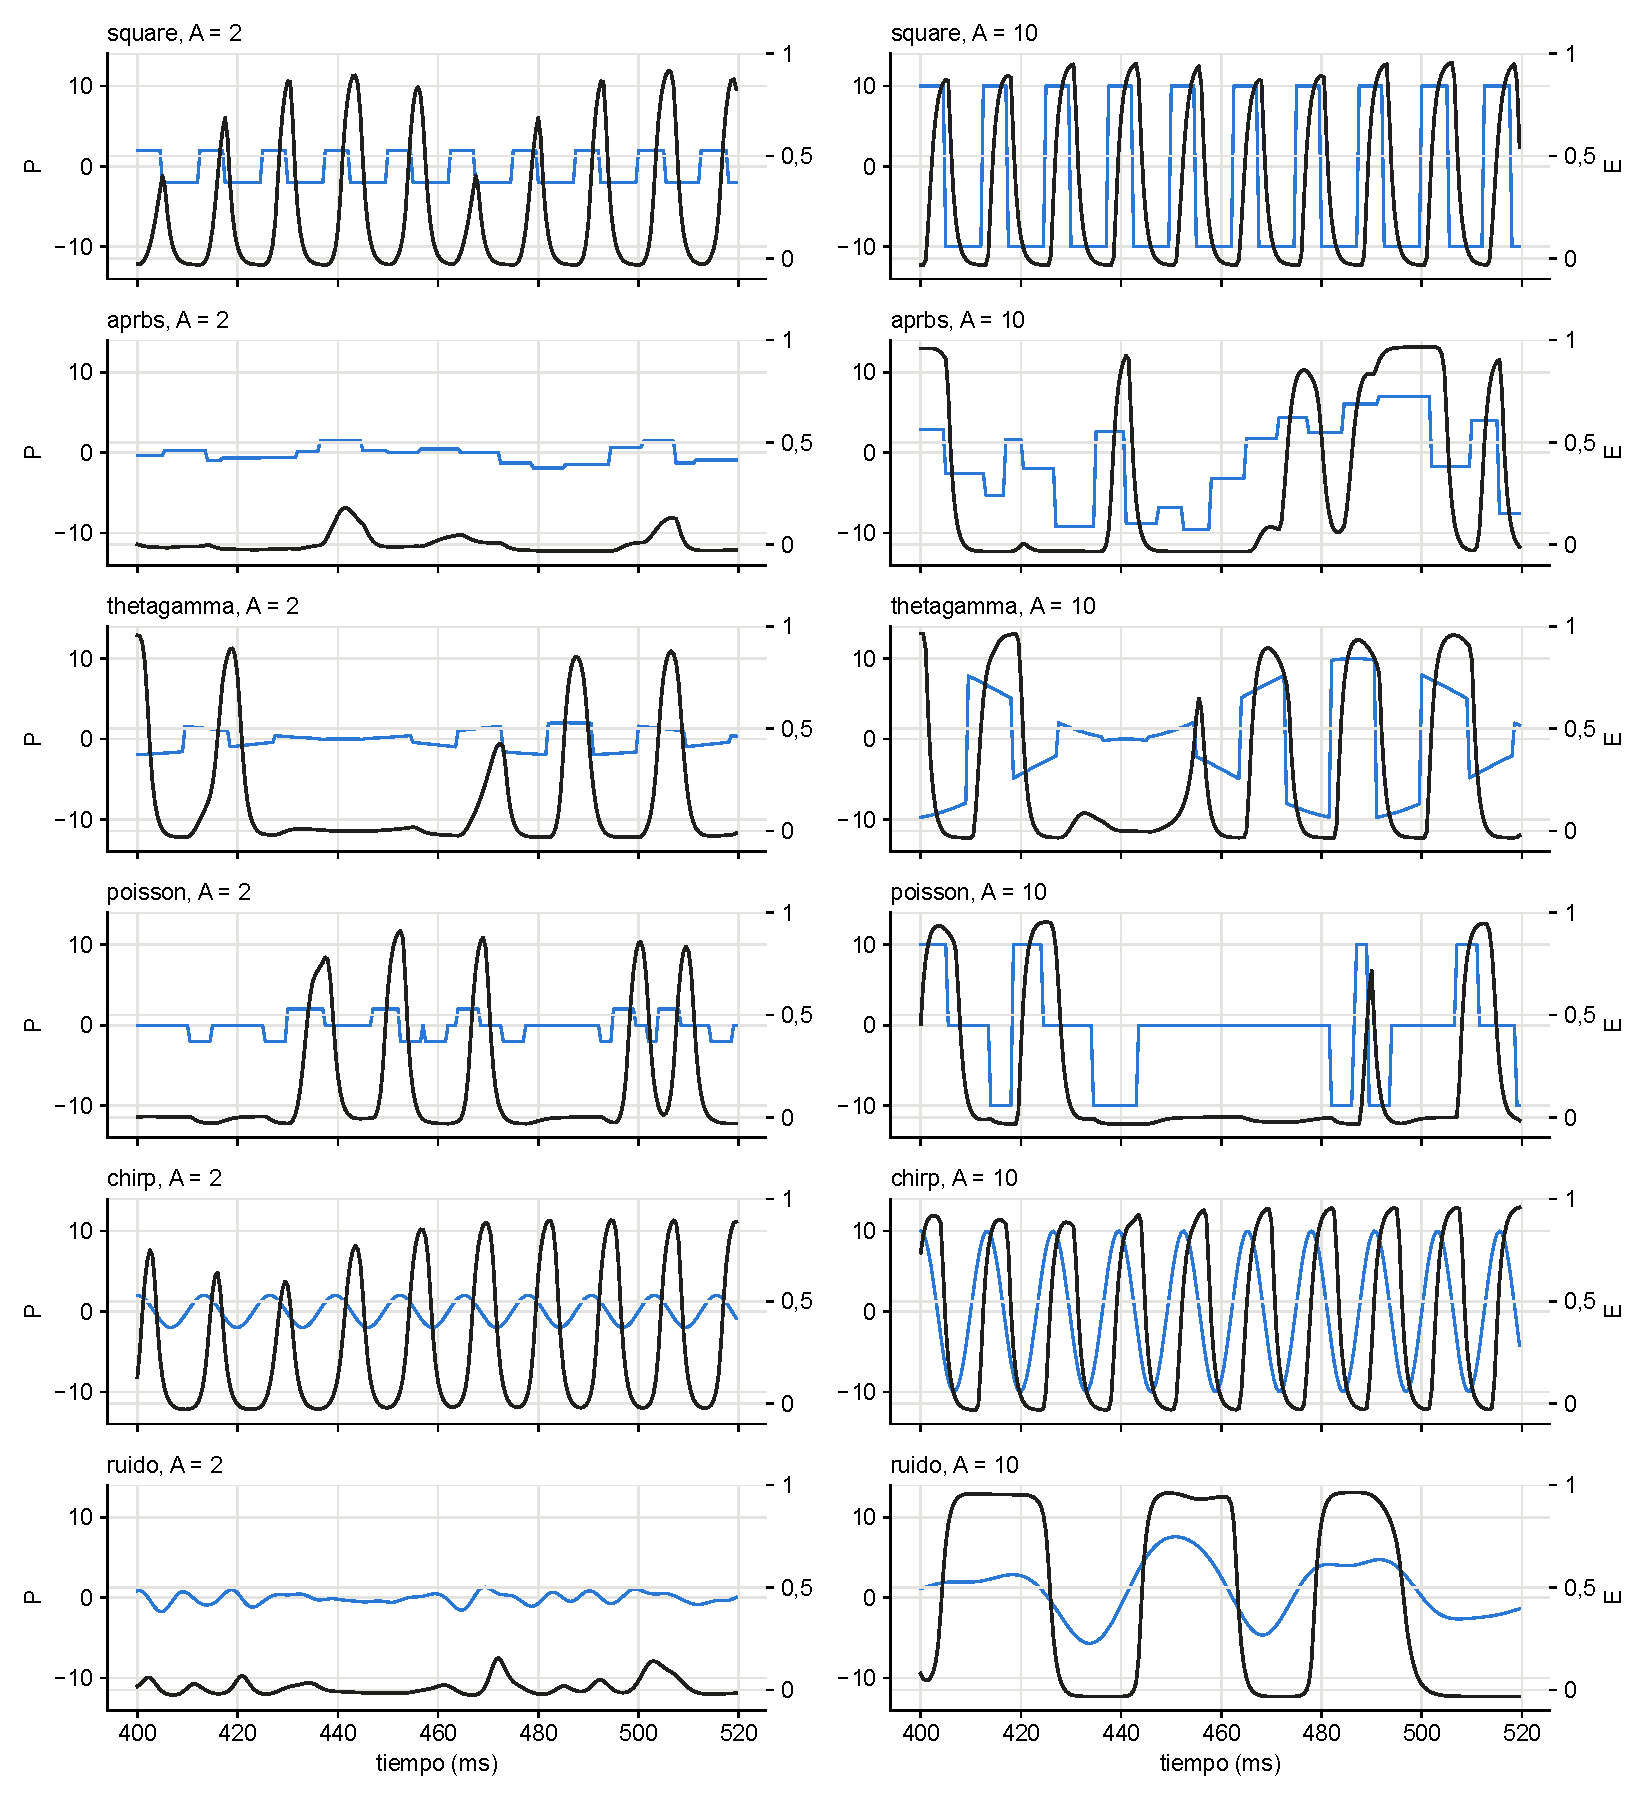
\includegraphics[width=0.92\textwidth]{ejemplos_amplitud.pdf}
\caption{Comando $P$ (azul, eje izquierdo) y actividad $E$ del simulador con actuador con recorte (negro, eje derecho) para cada familia, con amplitud 2 (izquierda) y 10 (derecha), entre 400 y 520~ms.}
\end{figure}

Se entrenaron los mismos modelos que con los datos anteriores, con warm start desde el white-box y desde cero, los dos niveles de ruido y tres semillas (e25), la segunda etapa con x0 entrenable (e26) y la referencia black-box (e27). Son 180 corridas, hechas en otra computadora. Las 180 terminaron, y todas usaron datasets idénticos a los originales, verificado por hash. La mediana fue de 72 minutos por corrida.

Las tablas comparan cada modelo con el mismo modelo entrenado con los datos de $[0, 2]$ (e21 para el actuador, e16 para la refractaria). El NRMSE se da sobre dos conjuntos de test. Uno son los 13 escenarios que interpolan del dataset anterior, con comandos positivos de hasta 2, comunes a las dos tandas. El otro son los 12 escenarios nuevos, con amplitudes de 1,5 a 11,5.

\section{Lazo abierto, actuador con recorte}

\begin{figure}[H]
\centering
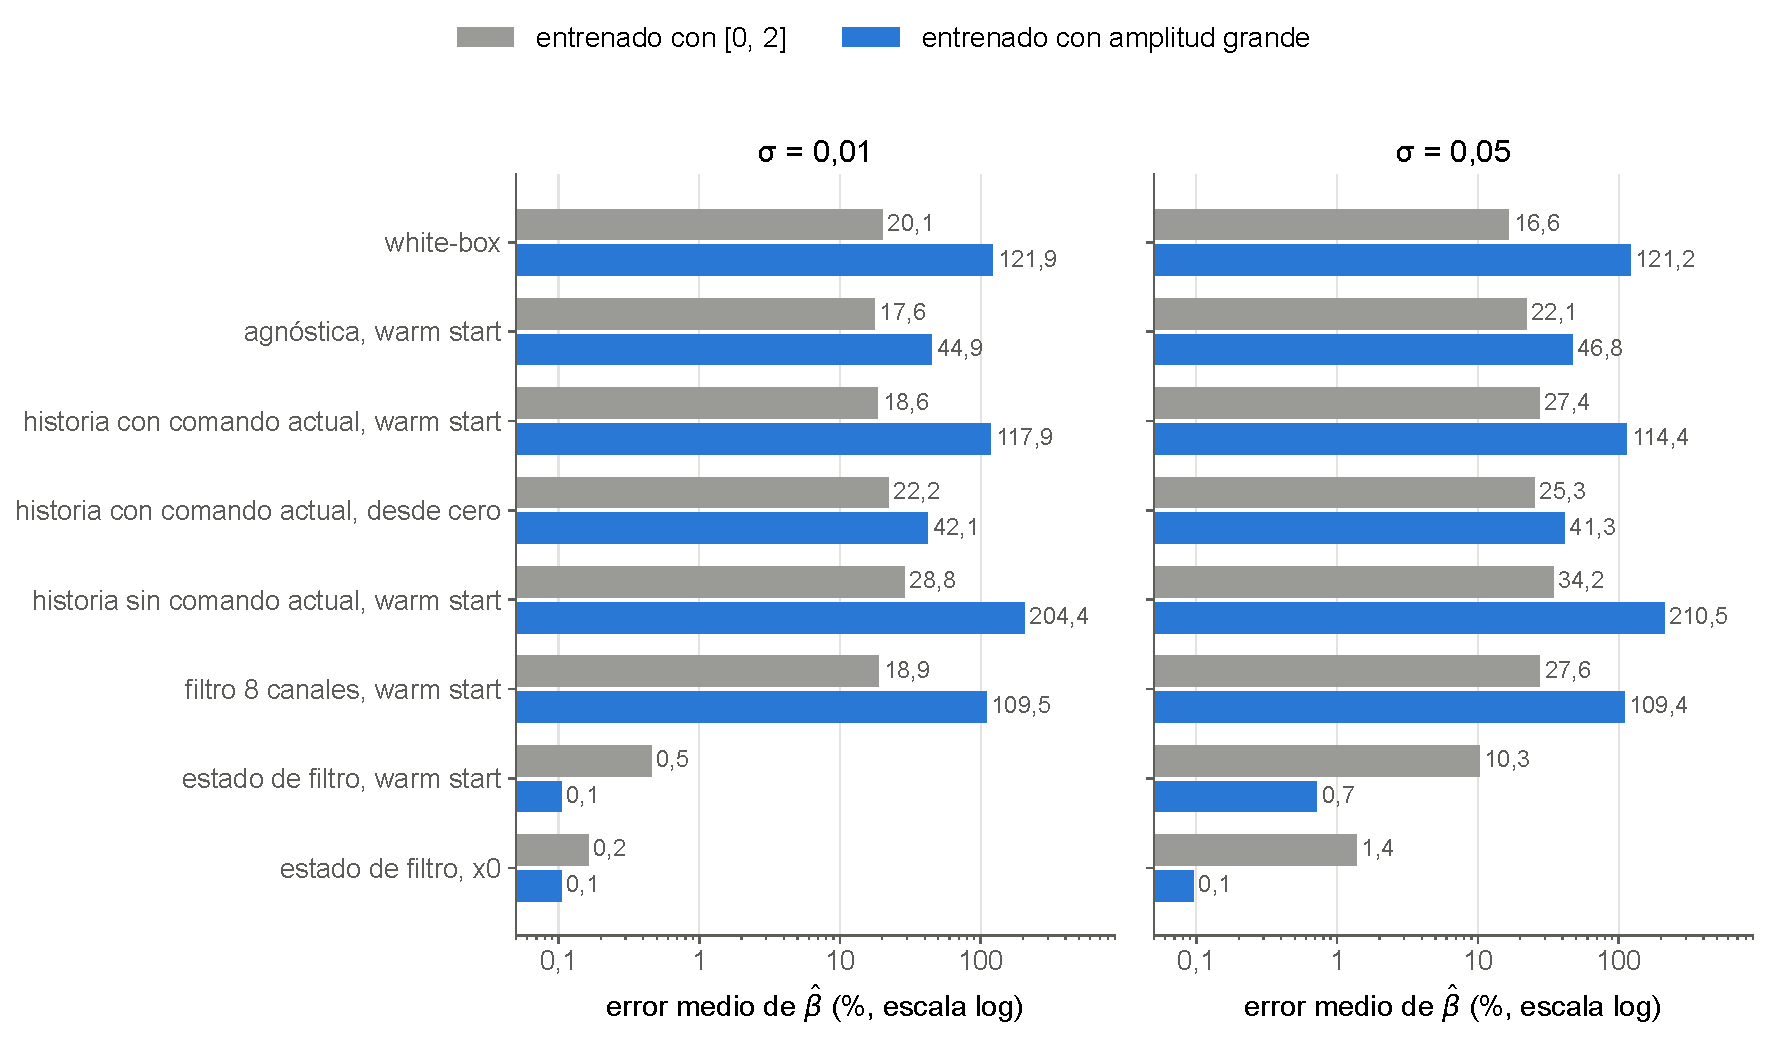
\includegraphics[width=\textwidth]{beta_actuador.pdf}
\caption{Error medio de los diez parámetros del actuador con recorte, entrenando con $[0, 2]$ (gris) y con amplitud grande (azul). Escala logarítmica. Media de tres semillas.}
\end{figure}

\begin{center}
\small
\begin{tabular}{@{}lcccc@{}}
\toprule
modelo, $\sigma = 0{,}01$ & error de $\bh$ (\%) & R² & NRMSE test anterior & NRMSE test nuevo \\
\midrule
white-box & 20,1 $\to$ 121,9 & $-$ & 7,28 $\to$ 23,85 & 10,28 \\
agnóstica, warm start & 17,6 $\to$ 44,9 & $-0{,}02 \to 0{,}00$ & 7,34 $\to$ 26,93 & 8,12 \\
historia con comando actual, warm start & 18,6 $\to$ 117,9 & $0{,}17 \to -0{,}03$ & 4,07 $\to$ 4,95 & 1,62 \\
historia con comando actual, desde cero & 22,2 $\to$ 42,1 & $-0{,}18 \to 0{,}25$ & 4,52 $\to$ 4,52 & 1,74 \\
historia sin comando actual, warm start & 28,8 $\to$ 204,4 & $-0{,}73 \to -0{,}62$ & 4,06 $\to$ 5,11 & 1,86 \\
filtro 8 canales, warm start & 18,9 $\to$ 109,5 & $0{,}13 \to -0{,}08$ & 4,23 $\to$ 4,18 & 1,31 \\
filtro 8 canales, desde cero & 30,0 $\to$ 43,7 & $-0{,}34 \to 0{,}19$ & 5,21 $\to$ 4,00 & 1,38 \\
estado de filtro, warm start & 0,46 $\to$ 0,10 & $1{,}000 \to 1{,}000$ & 2,25 $\to$ 2,25 & 0,37 \\
estado de filtro, x0 & 0,16 $\to$ 0,10 & $1{,}000 \to 1{,}000$ & 2,22 $\to$ 2,25 & 0,37 \\
black-box & $-$ & $-$ & 6,50 $\to$ 9,99 & 4,71 \\
black-box con historia & $-$ & $-$ & 3,47 $\to$ 3,97 & 1,09 \\
\bottomrule
\end{tabular}
\end{center}

Con comandos de hasta $\pm 12$, el recorte en $\pm 3$ actúa en buena parte del entrenamiento. Lo que le falta al modelo ya no es solo un filtro, sino además una saturación que corta el comando a un cuarto en los escenarios de mayor amplitud.

El estado de filtro, que tiene esa estructura, identifica todo. El error de $\bh$ es 0,10~\% con $\sigma = 0{,}01$ y 0,72~\% con $\sigma = 0{,}05$, que baja a 0,10~\% con x0 entrenable. La constante del filtro sale en $\hat\tau = 0{,}993$~ms. El nivel del recorte, que con los datos anteriores no se podía identificar y quedaba en su valor inicial de 10, ahora sale entre 2,99 y 3,01 en todas las semillas y niveles de ruido.

Los modelos sin el recorte en su estructura compensan la saturación deformando los parámetros. El white-box llega a 122~\% de error de $\bh$, y las correcciones con red con warm start a entre 110 y 204~\%, porque arrancan de ese white-box. Desde cero quedan entre 42 y 71~\%. En el test nuevo, las correcciones con historia reproducen bien (NRMSE de 1,3 a 1,9) con parámetros que no tienen relación con los verdaderos. En el test anterior, de amplitud chica, el white-box y la agnóstica empeoran mucho (de 7,3 a 24 y 27), porque sus parámetros quedaron ajustados al régimen saturado.

La black-box con historia es el mejor modelo sin la forma exacta en el test nuevo (1,09). La black-box sin historia queda en 4,71.

\begin{figure}[H]
\centering
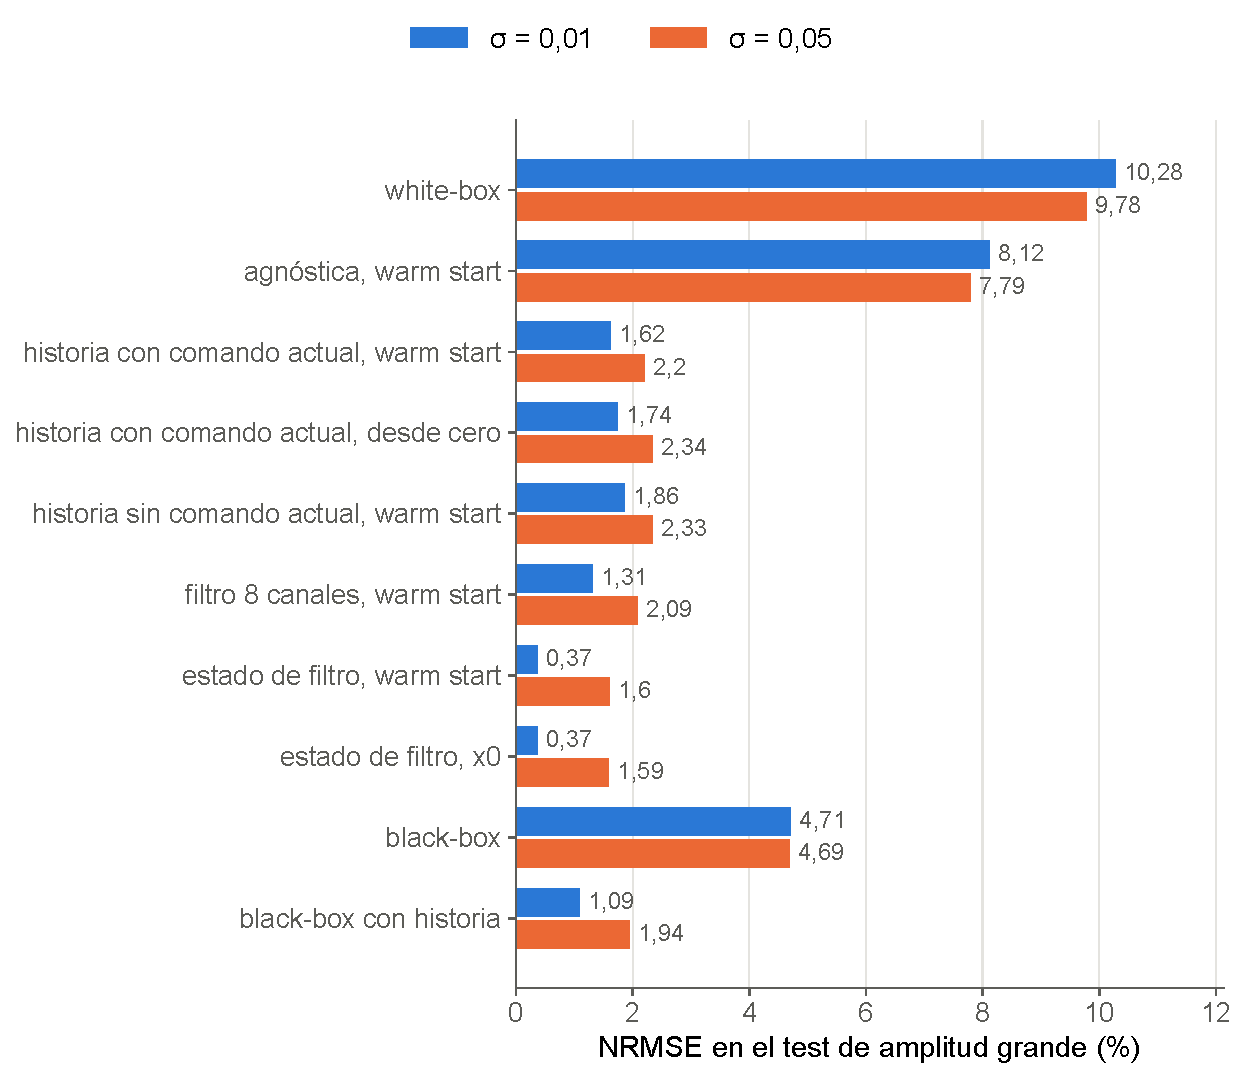
\includegraphics[width=0.75\textwidth]{nrmse_nuevo_actuador.pdf}
\caption{NRMSE en los 12 escenarios de test de amplitud grande, actuador con recorte. Media de tres semillas.}
\end{figure}

\section{Lazo abierto, refractaria}

\begin{figure}[H]
\centering
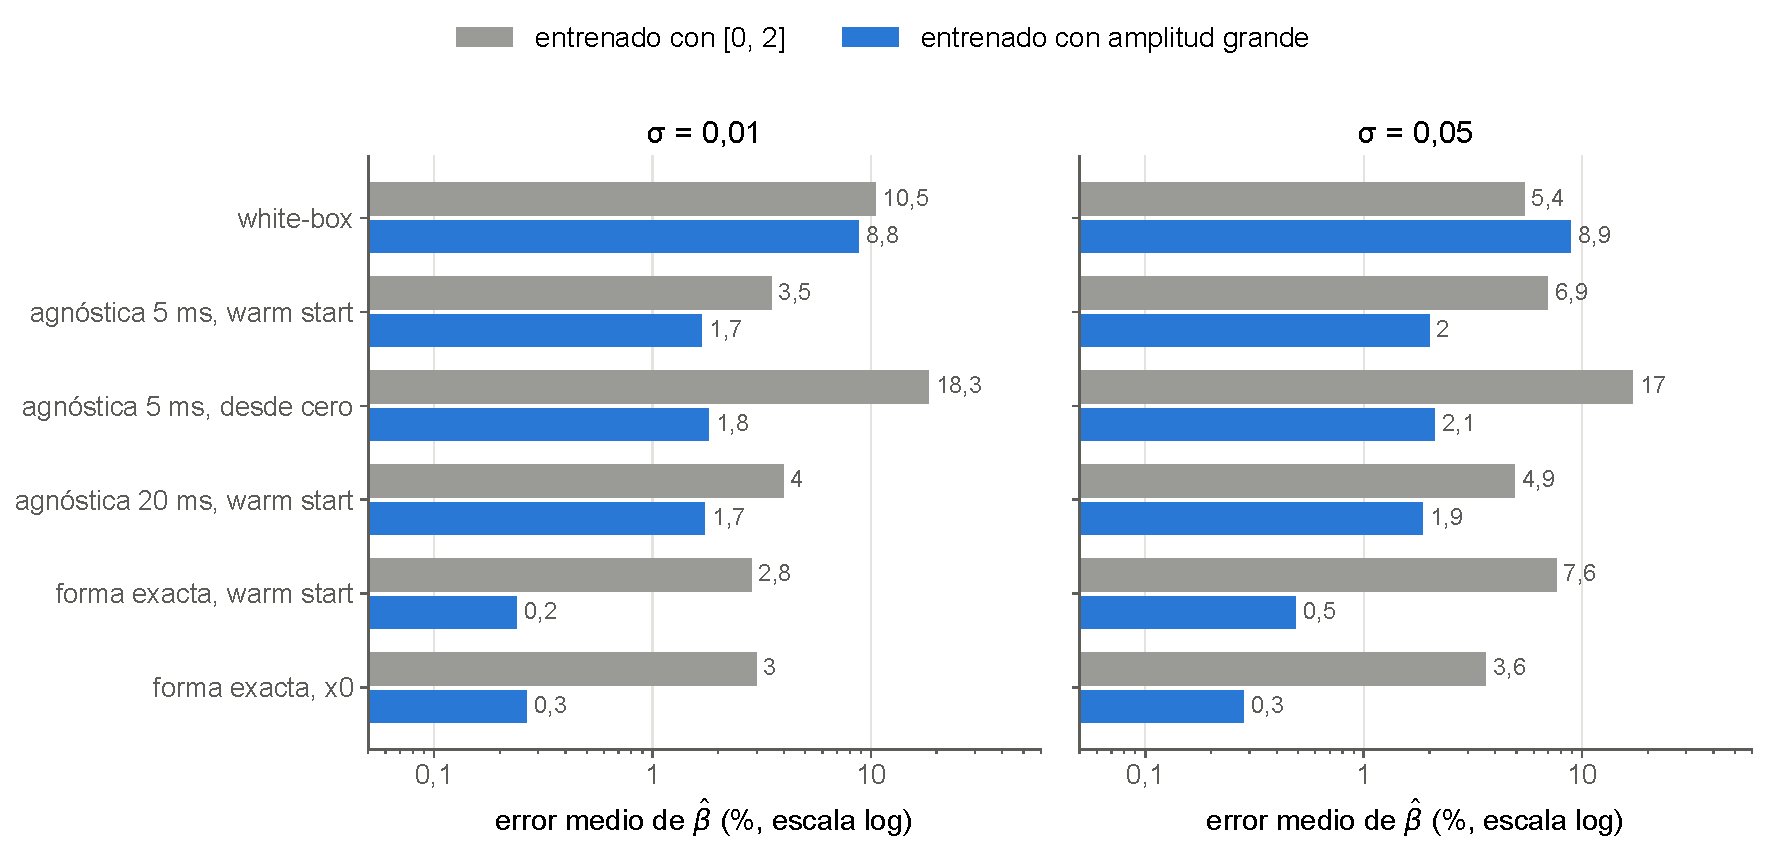
\includegraphics[width=\textwidth]{beta_refractaria.pdf}
\caption{Error medio de los diez parámetros de la planta refractaria, entrenando con $[0, 2]$ (gris) y con amplitud grande (azul). Escala logarítmica. Media de tres semillas.}
\end{figure}

\begin{center}
\small
\begin{tabular}{@{}lcccc@{}}
\toprule
modelo, $\sigma = 0{,}01$ & error de $\bh$ (\%) & R² & NRMSE test anterior & NRMSE test nuevo \\
\midrule
white-box & 10,5 $\to$ 8,8 & $-$ & 3,29 $\to$ 9,45 & 2,51 \\
agnóstica 5~ms, warm start & 3,5 $\to$ 1,7 & $0{,}78 \to 0{,}87$ & 2,13 $\to$ 2,20 & 0,44 \\
agnóstica 5~ms, desde cero & 18,3 $\to$ 1,8 & $0{,}42 \to 0{,}87$ & 2,28 $\to$ 2,37 & 0,46 \\
agnóstica 20~ms, warm start & 4,0 $\to$ 1,7 & $0{,}74 \to 0{,}87$ & 2,14 $\to$ 2,18 & 0,44 \\
forma exacta, warm start & 2,8 $\to$ 0,24 & $0{,}97 \to 1{,}00$ & 2,14 $\to$ 2,12 & 0,38 \\
forma exacta, x0 & 3,0 $\to$ 0,26 & $0{,}97 \to 1{,}00$ & 2,13 $\to$ 2,12 & 0,38 \\
black-box & $-$ & $-$ & 2,88 $\to$ 2,68 & 0,60 \\
black-box con historia & $-$ & $-$ & 3,20 $\to$ 3,13 & 0,83 \\
\bottomrule
\end{tabular}
\end{center}

En la planta refractaria todo mejora. El término refractario crece con la actividad, y con comandos grandes la población pasa más tiempo con actividad alta, donde el término es grande y se distingue del resto. La agnóstica identifica $\beta$ con 1,7~\% de error, y llega a lo mismo desde cero (1,8~\%, antes 18~\%), así que el warm start deja de ser necesario. La forma exacta baja a 0,24~\%. El R² de la agnóstica sube de 0,78 a 0,87. El white-box mejora poco en $\bh$ y empeora en el test anterior, como en el actuador.

\section{Planta ideal y sesgo por ventanas}

El white-box sobre la planta ideal tiene 0,27~\% de error de $\bh$ con $\sigma = 0{,}01$ y 0,63~\% con $\sigma = 0{,}05$. Con los datos de amplitud chica, el mismo modelo tenía 9,8~\% con $\sigma = 0{,}05$, por el ruido en el estado inicial de cada ventana. Con comandos grandes la respuesta es mucho mayor que el ruido, y ese sesgo casi desaparece. Por eso x0 entrenable cambia poco en esta tanda, salvo en el estado de filtro con $\sigma = 0{,}05$.

\section{Lazo cerrado}

Cada modelo reemplaza al simulador bajo el controlador del paper sin cambios. La distancia es la diferencia eficaz entre las trayectorias de $E$ e $I$ del lazo con el modelo y del lazo con el simulador, sobre el último 80~\% de la corrida. Los valores son medianas de tres semillas con $\sigma = 0{,}01$. La black-box entra por primera vez al lazo cerrado.

\begin{figure}[H]
\centering
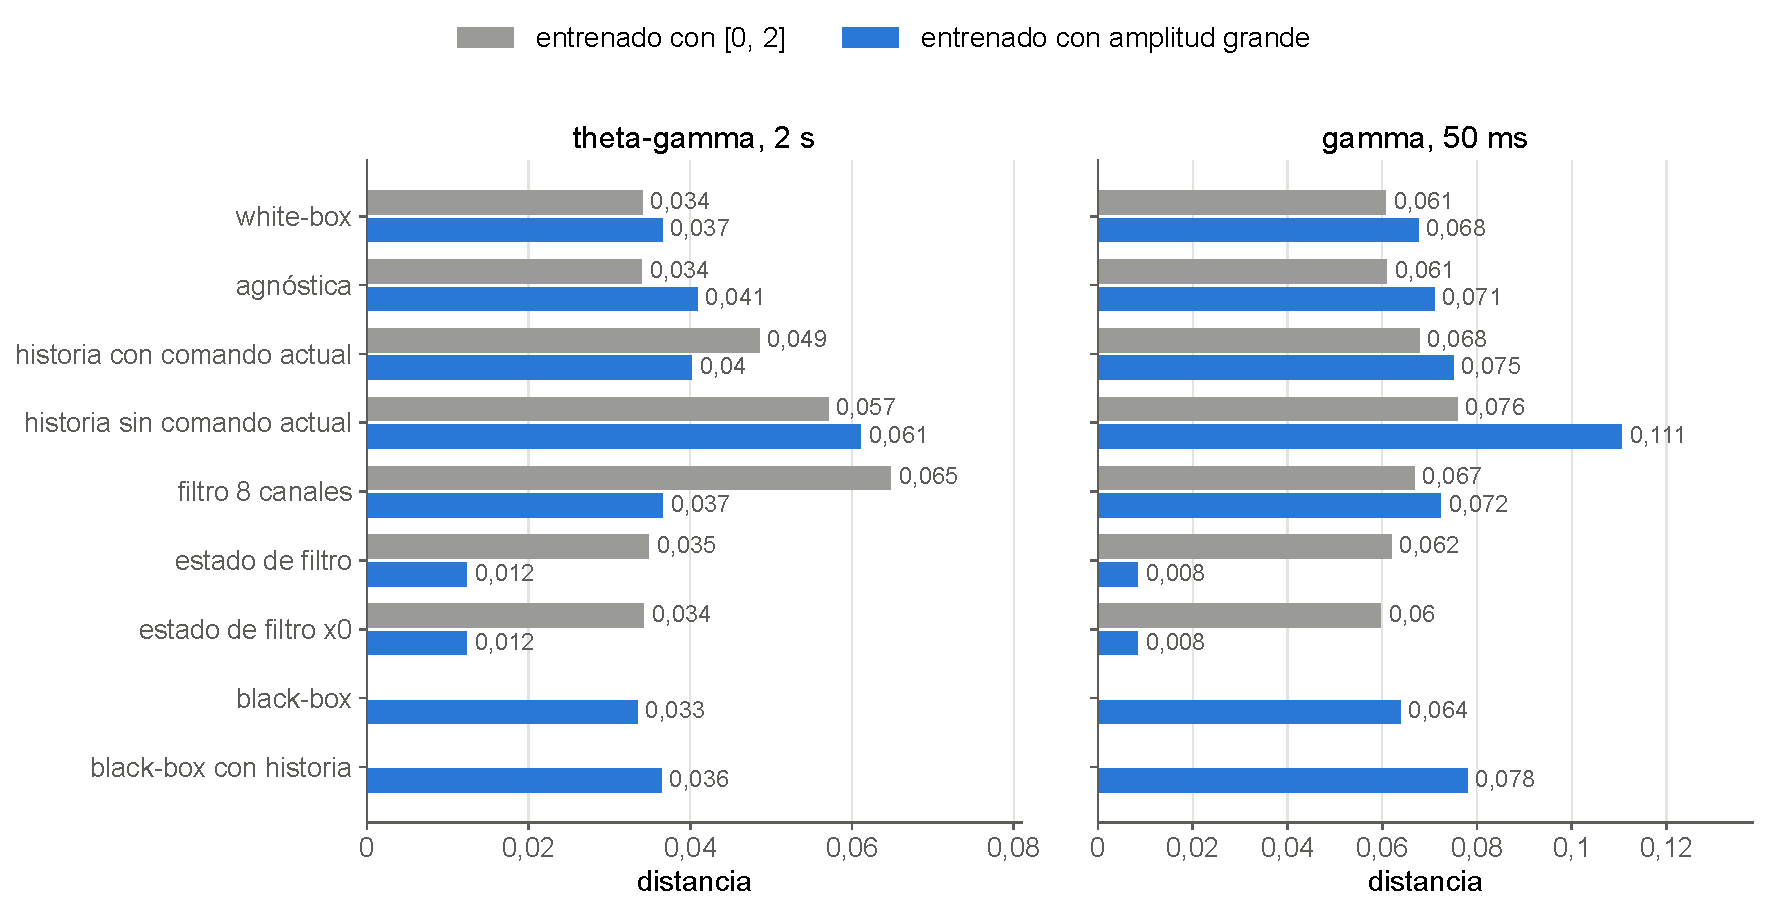
\includegraphics[width=\textwidth]{distancia_lazos_amplitud.pdf}
\caption{Distancia al lazo con el simulador con actuador con recorte, $\sigma = 0{,}01$, modelos entrenados con $[0, 2]$ (gris) y con amplitud grande (azul). El estado de filtro entrenado con $[0, 2]$ es el que conserva el recorte en $\pm 10$.}
\end{figure}

\begin{center}
\small
\begin{tabular}{@{}lcccc@{}}
\toprule
actuador con recorte, $\sigma = 0{,}01$ & theta-gamma & gamma 50~ms & theta en rango & gamma en rango \\
\midrule
white-box & 0,034 $\to$ 0,037 & 0,061 $\to$ 0,068 & 0,001 $\to$ 0,007 & 0,003 $\to$ 0,021 \\
agnóstica & 0,034 $\to$ 0,041 & 0,061 $\to$ 0,071 & 0,001 $\to$ 0,008 & 0,003 $\to$ 0,008 \\
historia con comando actual & 0,049 $\to$ 0,040 & 0,068 $\to$ 0,075 & 0,029 $\to$ 0,020 & 0,044 $\to$ 0,030 \\
historia sin comando actual & 0,057 $\to$ 0,061 & 0,076 $\to$ 0,111 & 0,035 $\to$ 0,072 & 0,055 $\to$ 0,061 \\
filtro 8 canales & 0,065 $\to$ 0,037 & 0,067 $\to$ 0,072 & 0,047 $\to$ 0,004 & 0,053 $\to$ 0,003 \\
estado de filtro & 0,035 $\to$ 0,012 & 0,062 $\to$ 0,008 & 0,000 $\to$ 0,000 & 0,000 $\to$ 0,000 \\
black-box & $-$ $\to$ 0,033 & $-$ $\to$ 0,064 & $-$ $\to$ 0,002 & $-$ $\to$ 0,004 \\
black-box con historia & $-$ $\to$ 0,036 & $-$ $\to$ 0,078 & $-$ $\to$ 0,003 & $-$ $\to$ 0,004 \\
\bottomrule
\end{tabular}
\end{center}

El estado de filtro entrenado con amplitud grande reproduce el lazo del simulador sin fijar ningún parámetro a mano, con distancia 0,012 en theta-gamma y 0,008 en gamma con $\sigma = 0{,}01$, y 0,013 con $\sigma = 0{,}05$. Con los datos anteriores hacía falta fijar el nivel del recorte en 3 y agregar x0 entrenable para llegar a eso.

Las correcciones con red siguen lejos del lazo del simulador en theta-gamma y gamma (entre 0,037 y 0,111). El filtro de 8 canales es el que más cambia: con las referencias en rango baja de 0,05 a 0,003 y ya no oscila en reposo. La historia sin comando actual empeora. El white-box y la agnóstica empeoran con las referencias en rango, porque sus parámetros quedaron ajustados al régimen saturado.

La black-box queda a la misma distancia que el white-box en theta-gamma y gamma (0,033 a 0,078), y cerca del simulador con las referencias en rango (0,002 a 0,004).

En la planta refractaria todos los modelos reproducen el lazo del simulador, con distancias de 0,000 (forma exacta) a 0,007 (white-box) en theta-gamma.

\subsection{Seguimiento de la referencia}

Referencia theta-gamma con ventana, $r_I(t) = T_w(t)\,[0{,}2\,\sin(2\pi f_\gamma t - 0{,}94) + 0{,}25]$ y $r_E(t) = T_w(t)\,[0{,}3\,\sin(2\pi f_\gamma t) + 0{,}45]$, con $f_\gamma = 120$~Hz.

\begin{figure}[H]
\centering
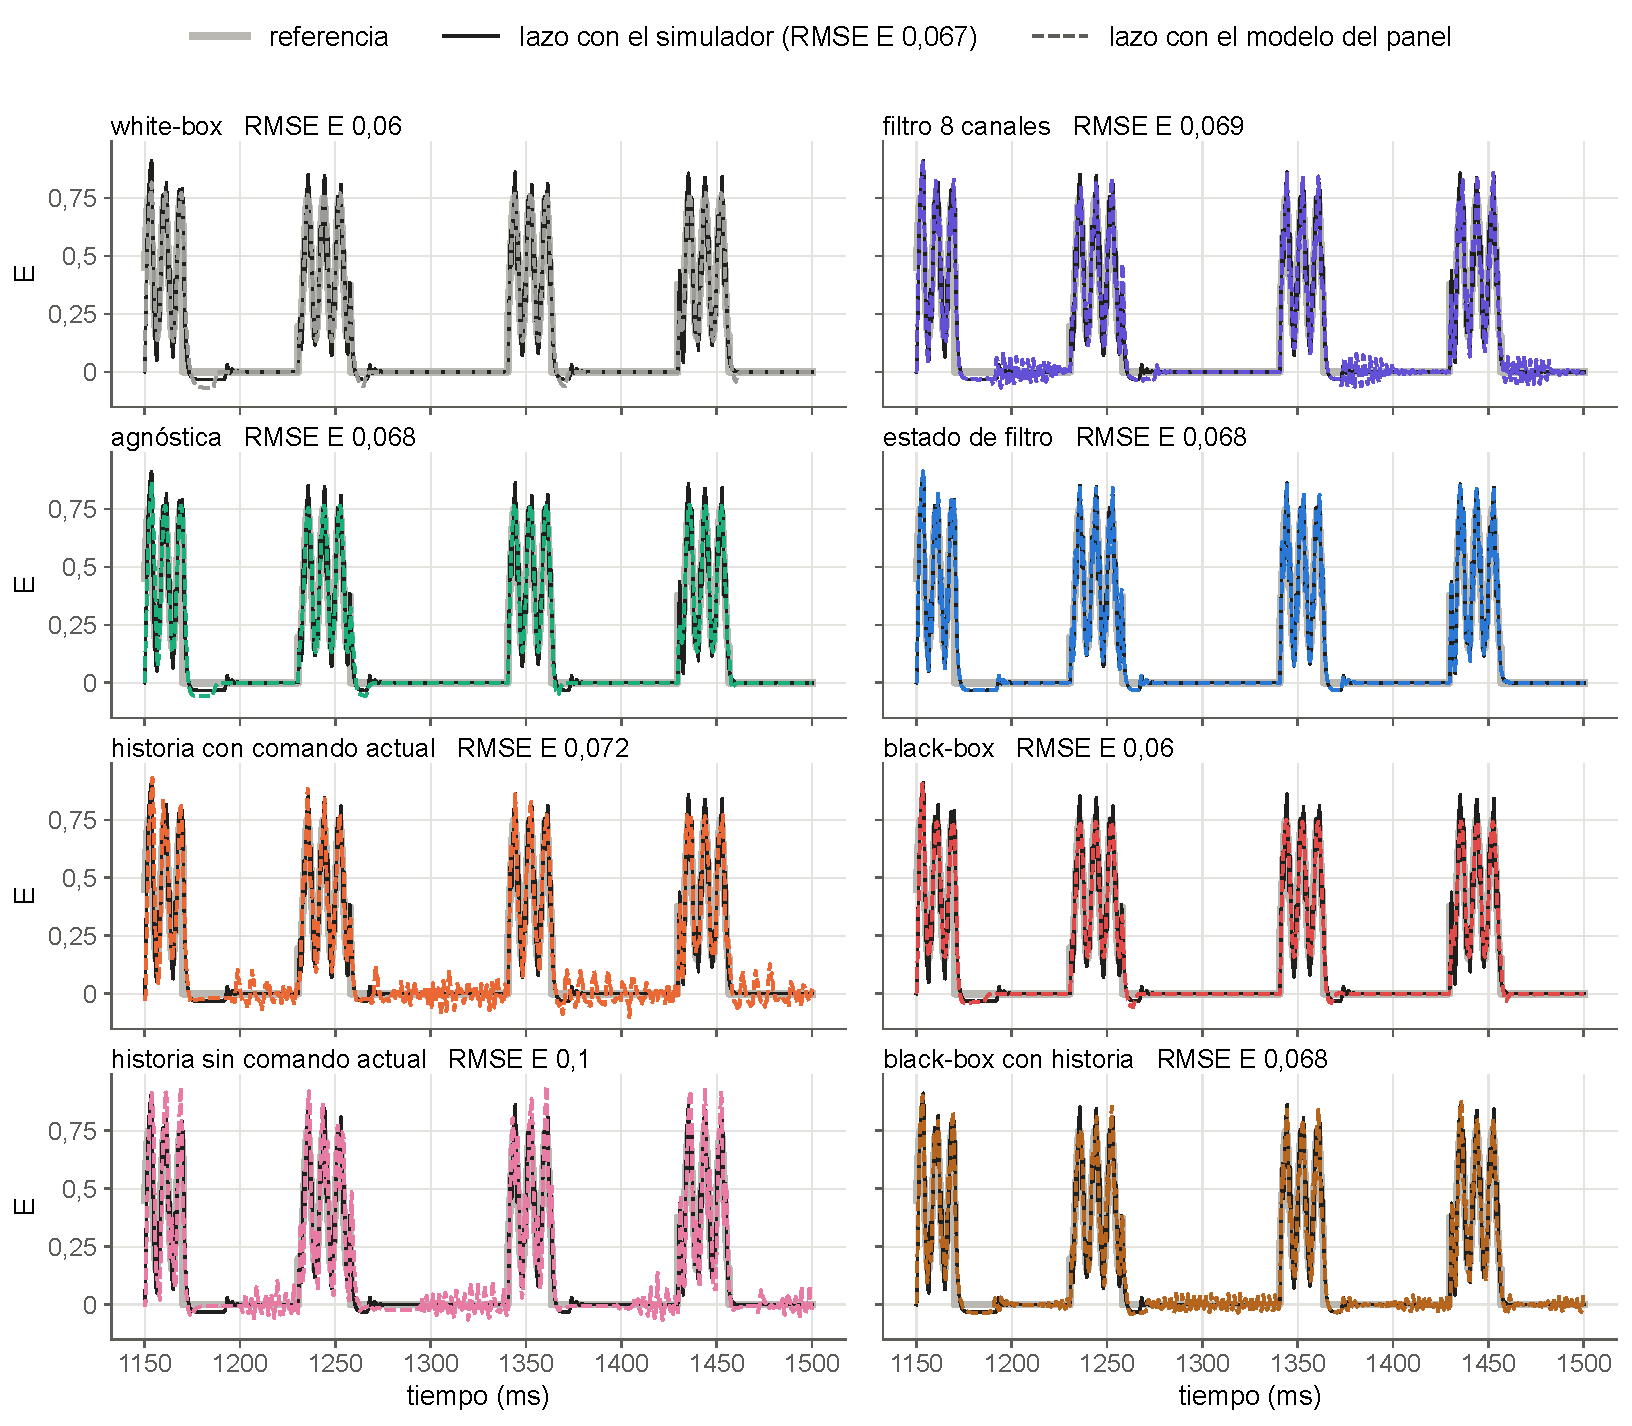
\includegraphics[width=\textwidth]{theta2s_E.pdf}
\caption{Actividad $E$ con la referencia theta-gamma, entre 1150 y 1500~ms. Gris, referencia. Negro, lazo con el simulador. Discontinua, lazo con el modelo del panel, entrenado con amplitud grande (semilla 0, $\sigma = 0{,}01$). En cada panel, RMSE contra la referencia.}
\end{figure}
\begin{figure}[H]
\centering
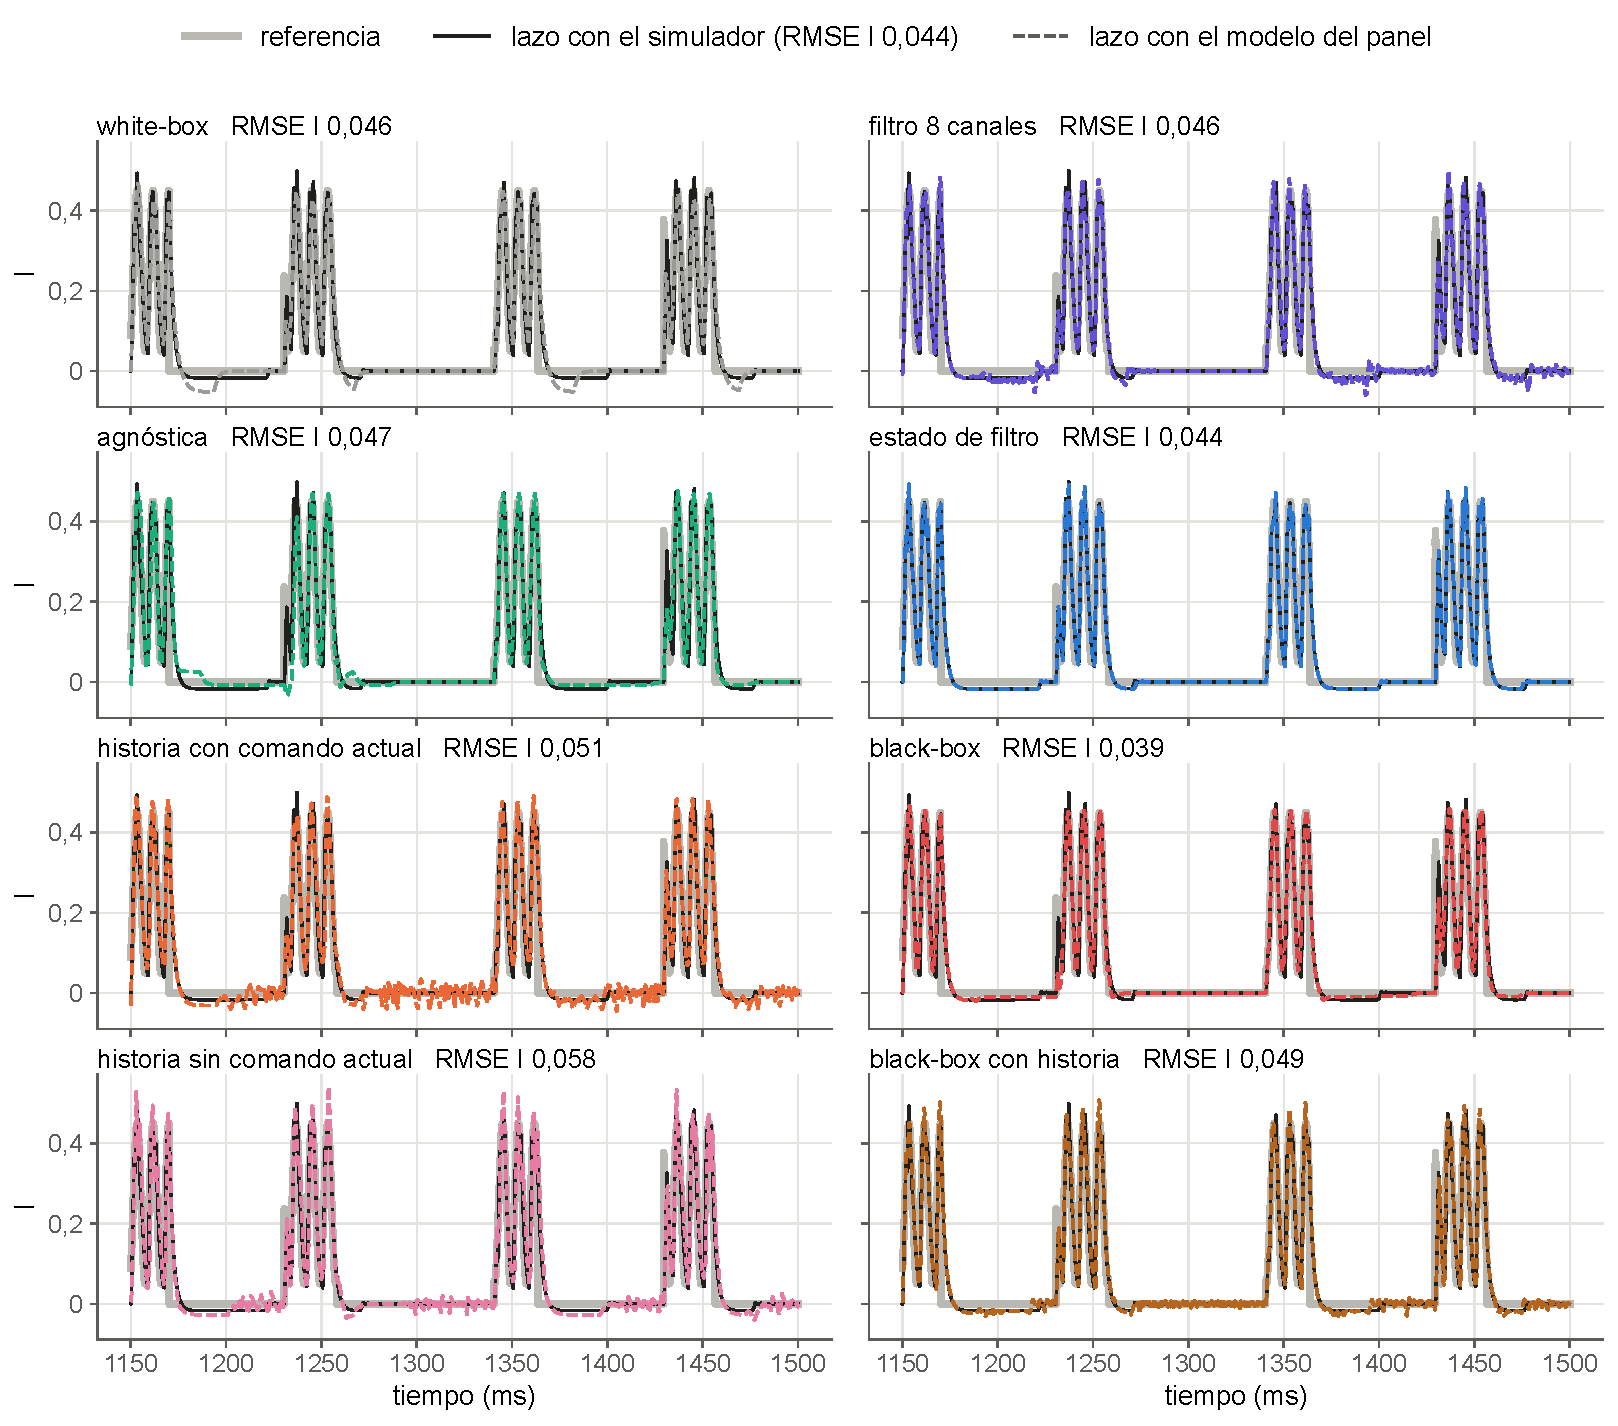
\includegraphics[width=\textwidth]{theta2s_I.pdf}
\caption{Actividad $I$ en las mismas corridas.}
\end{figure}
El estado de filtro se superpone al lazo con el simulador. El white-box, la agnóstica y la black-box siguen la forma de las ráfagas y se apartan en los picos. Las dos historias, el filtro de 8 canales y la black-box con historia siguen las ráfagas pero oscilan entre ellas, donde la referencia y el lazo con el simulador están en reposo. Las oscilaciones del filtro de 8 canales son más cortas que con los datos de $[0, 2]$.

Gamma continua, $r_I(t) = 0{,}2\,\sin(2\pi f_\gamma t - 0{,}94) + 0{,}25$ y $r_E(t) = 0{,}3\,\sin(2\pi f_\gamma t) + 0{,}45$, durante 50~ms.

\begin{figure}[H]
\centering
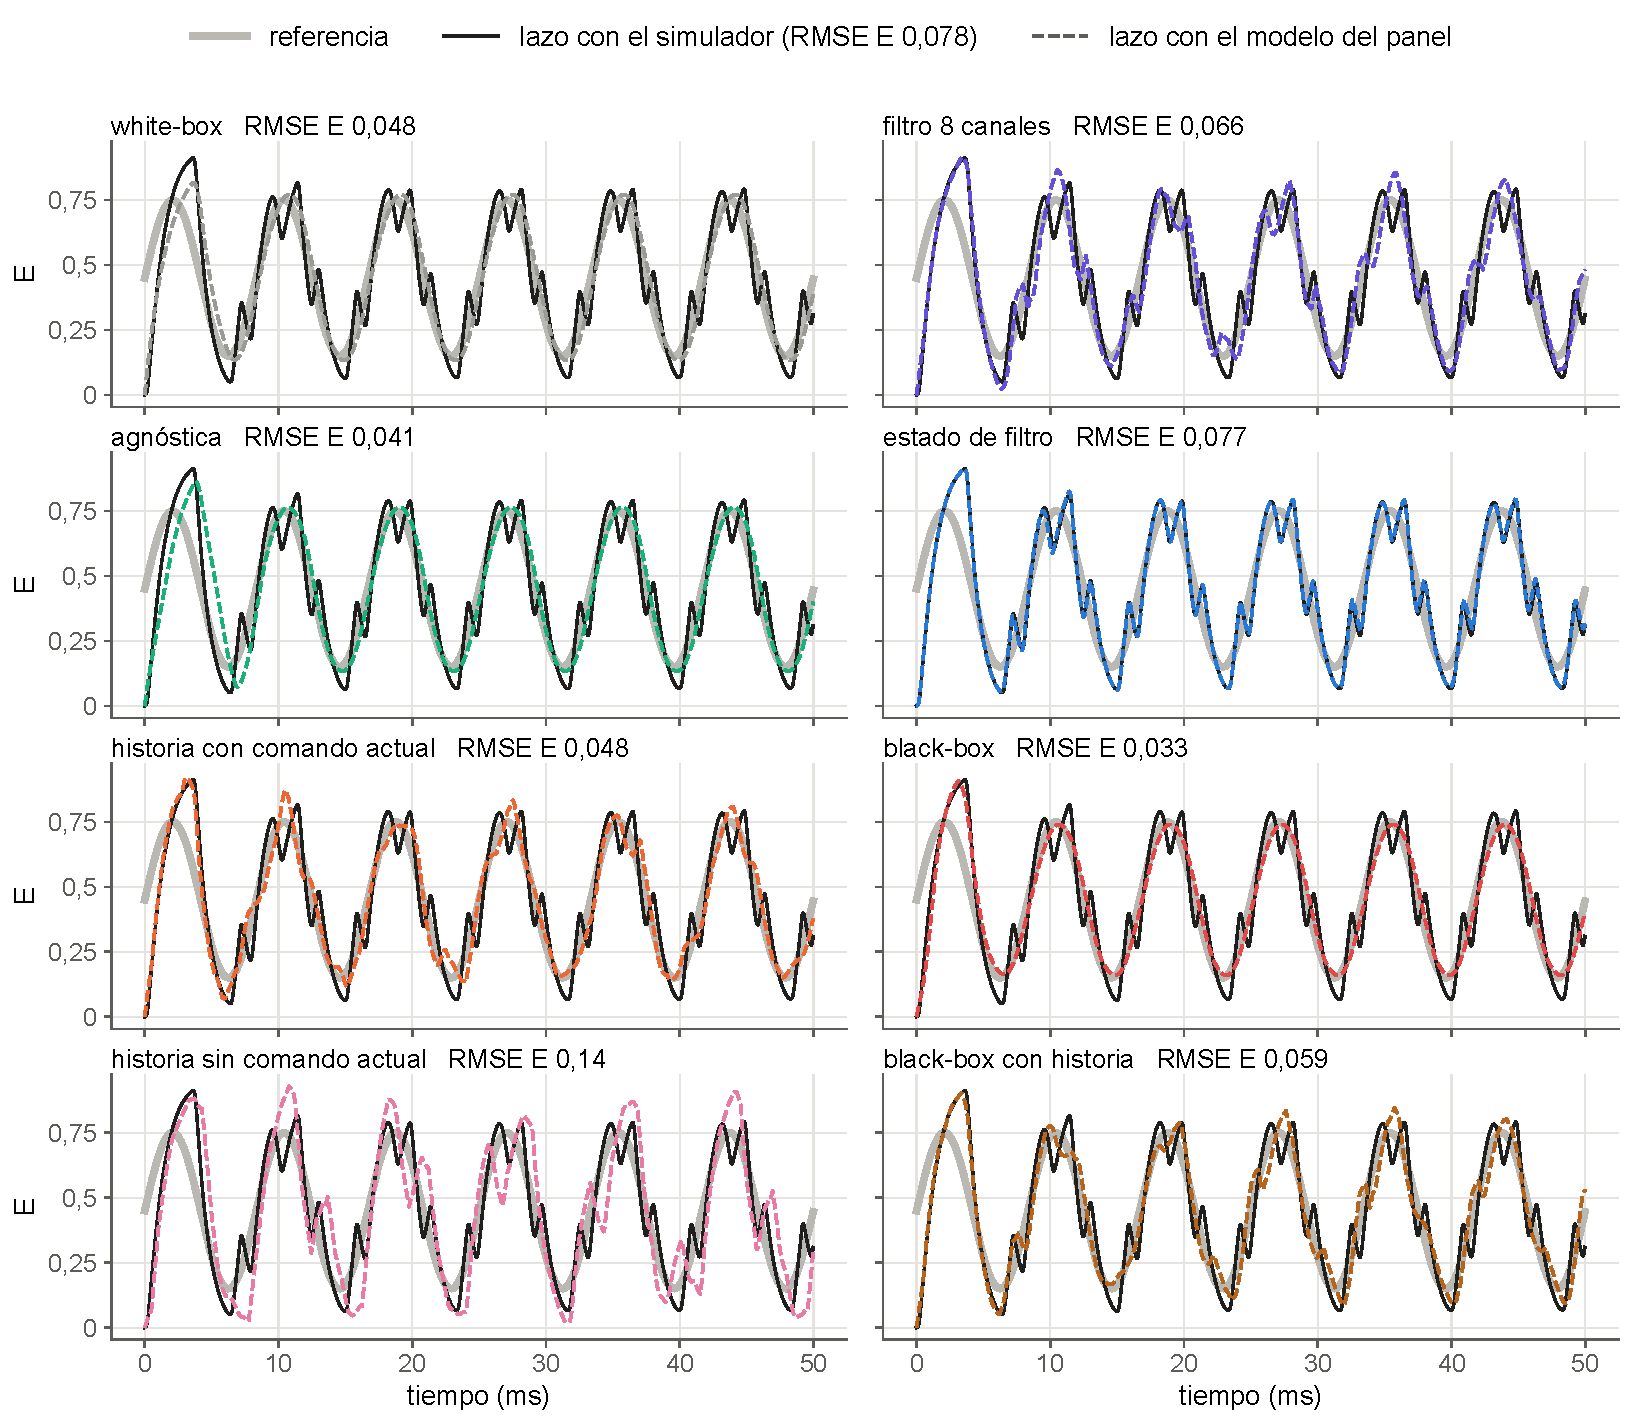
\includegraphics[width=\textwidth]{gamma50_E.pdf}
\caption{Actividad $E$ con la gamma continua de 50~ms. Gris, referencia. Negro, lazo con el simulador. Discontinua, lazo con el modelo del panel, entrenado con amplitud grande (semilla 0, $\sigma = 0{,}01$). En cada panel, RMSE contra la referencia.}
\end{figure}
\begin{figure}[H]
\centering
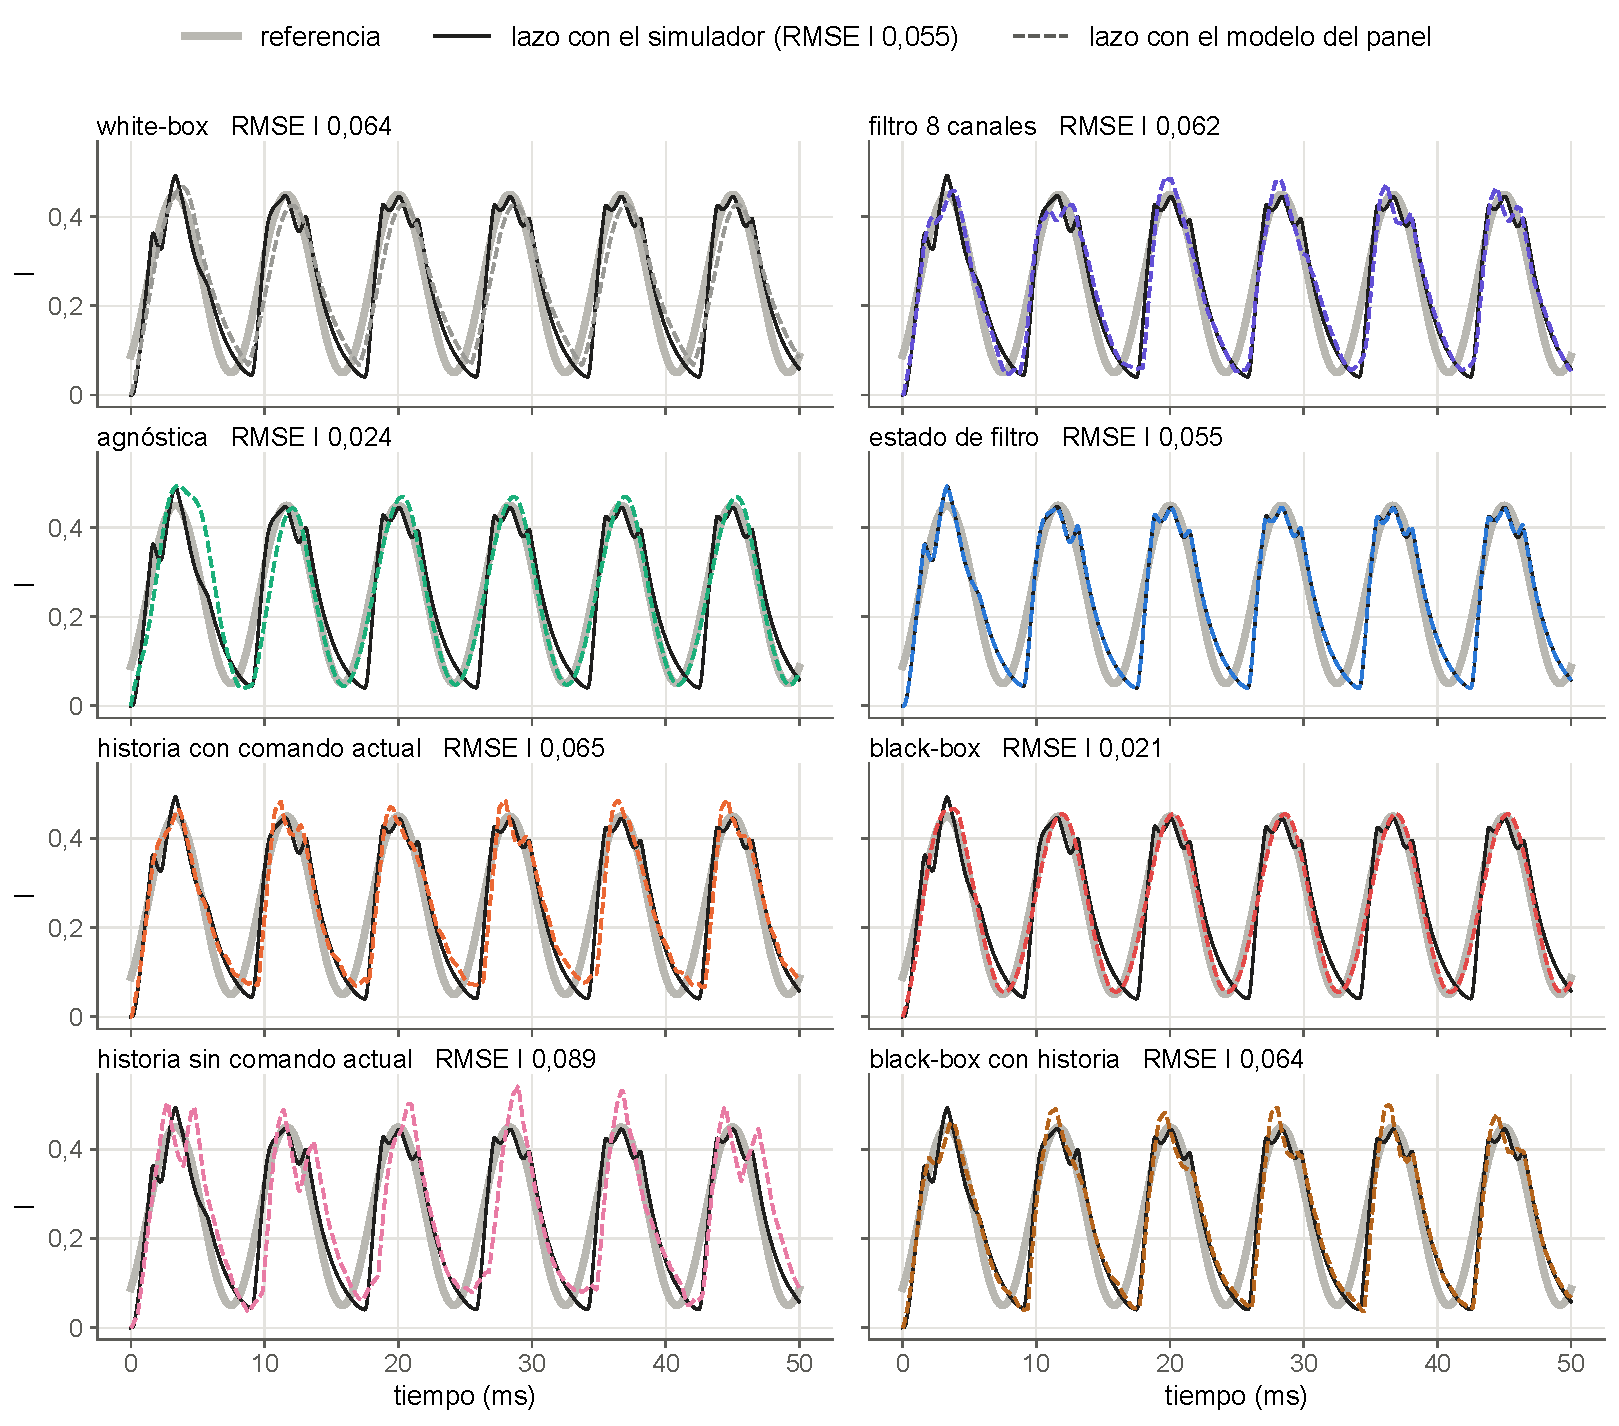
\includegraphics[width=\textwidth]{gamma50_I.pdf}
\caption{Actividad $I$ en las mismas corridas.}
\end{figure}
Con la gamma continua, el lazo con el simulador va atrasado respecto de la referencia, por el filtro del actuador. El estado de filtro reproduce ese atraso. La black-box y la agnóstica quedan en fase con la referencia (RMSE de 0,028 y 0,034 contra 0,068 del simulador). La historia sin comando actual se deforma (0,118).

Referencias en rango, $(r_I, r_E) = (I, E)$ del Wilson-Cowan sin perturbación con $P(t) = 1 + 0{,}8\,\sin(2\pi f t)$ y $Q(t) = 0{,}75 + 0{,}6\,\sin(2\pi f t - 1)$, con $f = 8$~Hz durante 500~ms y $f = 40$~Hz durante 250~ms.

\begin{figure}[H]
\centering
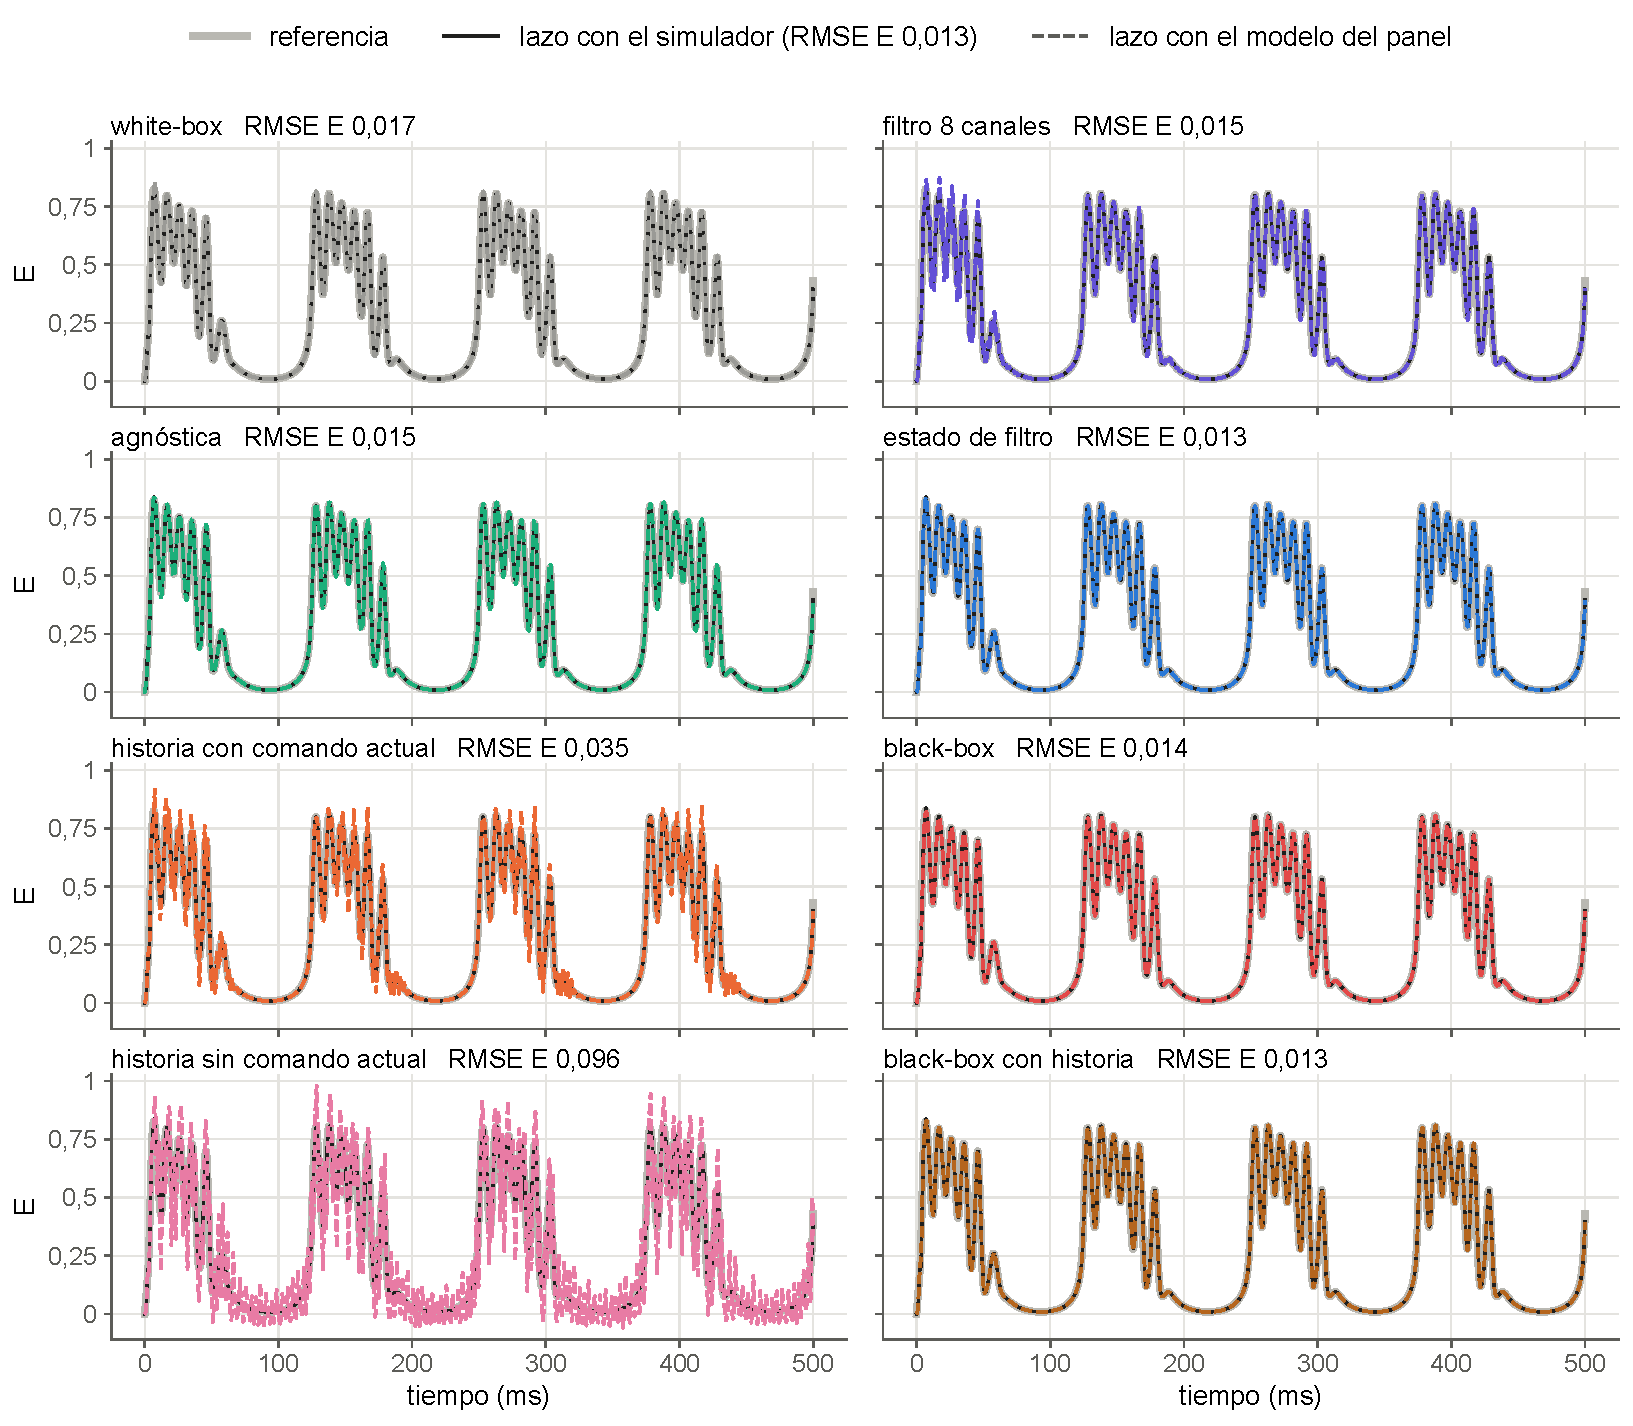
\includegraphics[width=\textwidth]{theta_rango_E.pdf}
\caption{Actividad $E$ con la referencia theta de 8~Hz en rango. Gris, referencia. Negro, lazo con el simulador. Discontinua, lazo con el modelo del panel, entrenado con amplitud grande (semilla 0, $\sigma = 0{,}01$). En cada panel, RMSE contra la referencia.}
\end{figure}
\begin{figure}[H]
\centering
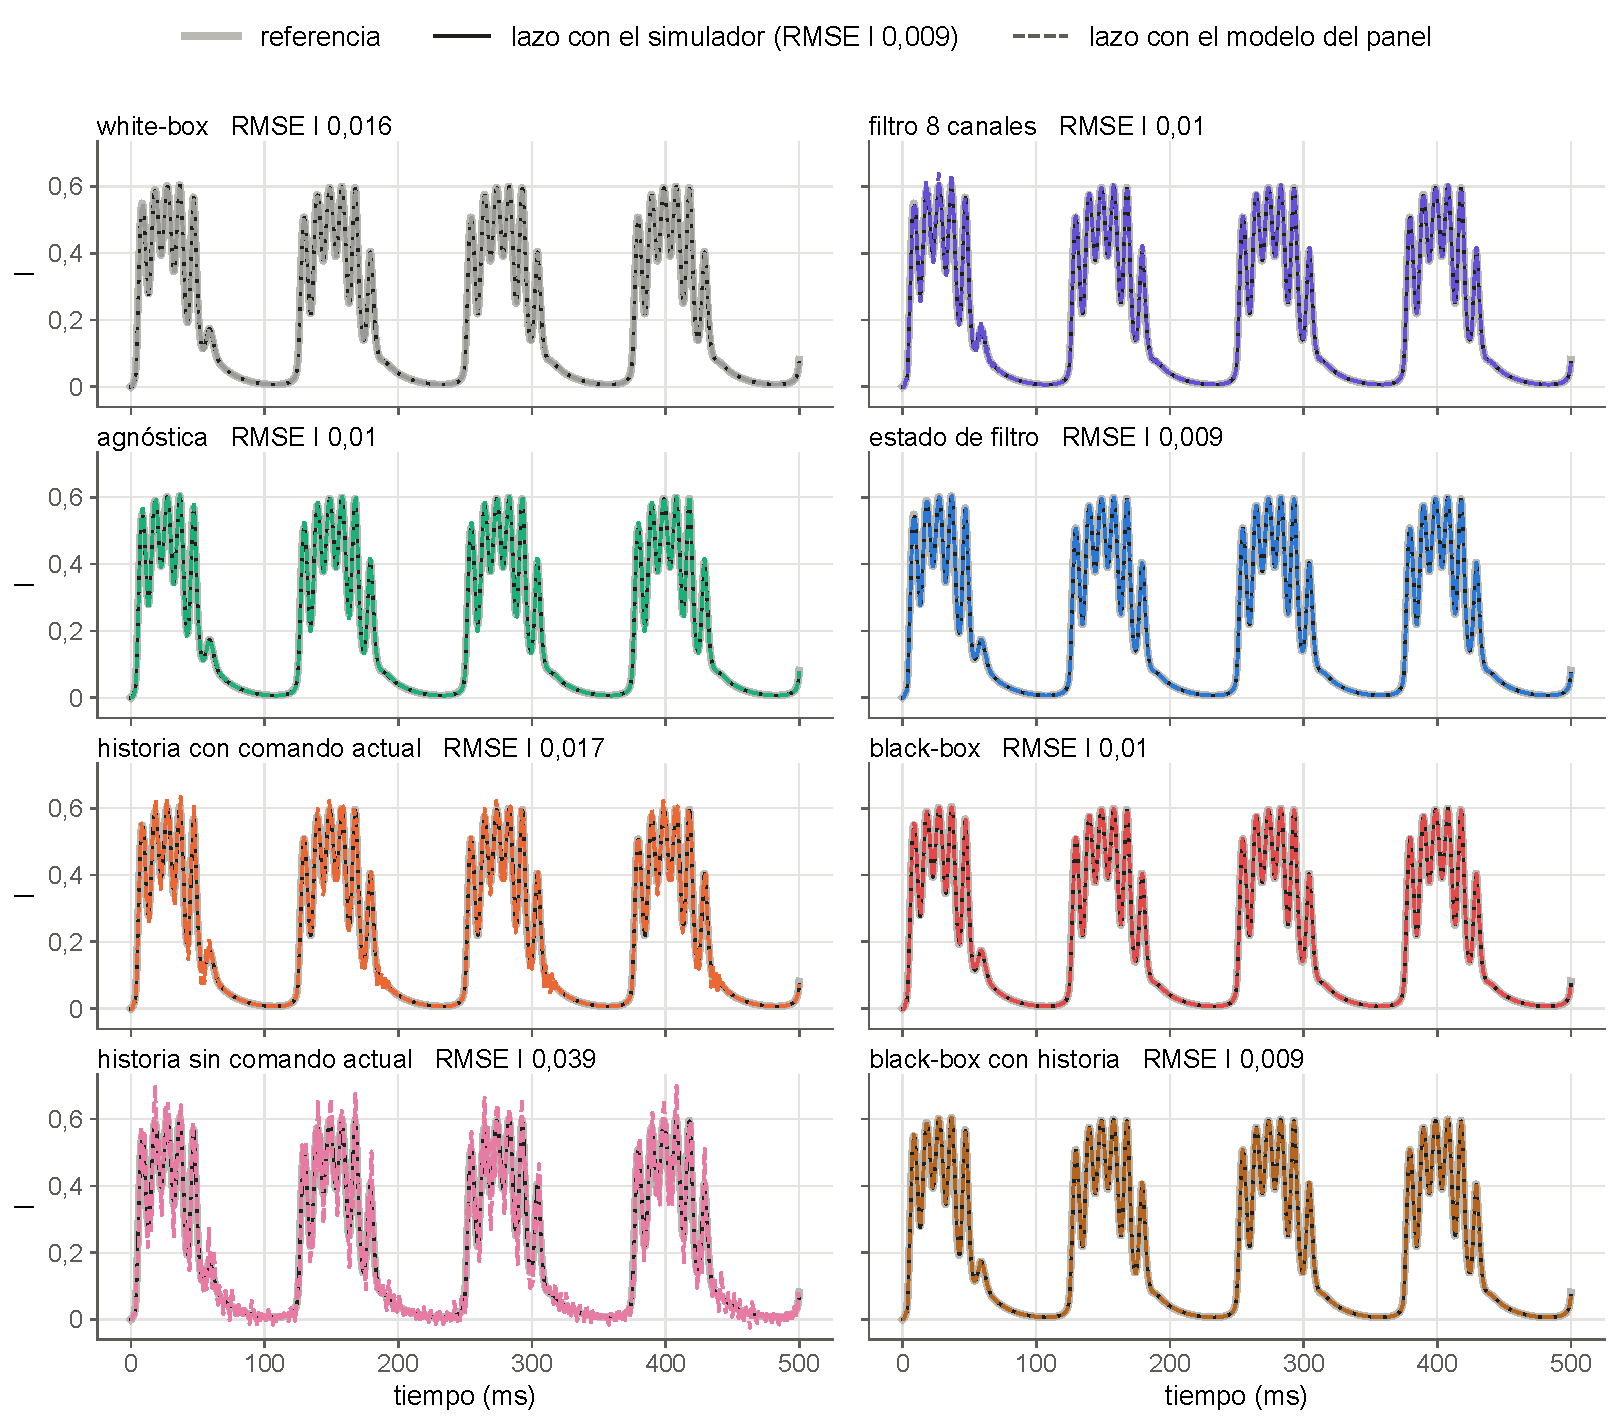
\includegraphics[width=\textwidth]{theta_rango_I.pdf}
\caption{Actividad $I$ con la referencia theta de 8~Hz en rango.}
\end{figure}
\begin{figure}[H]
\centering
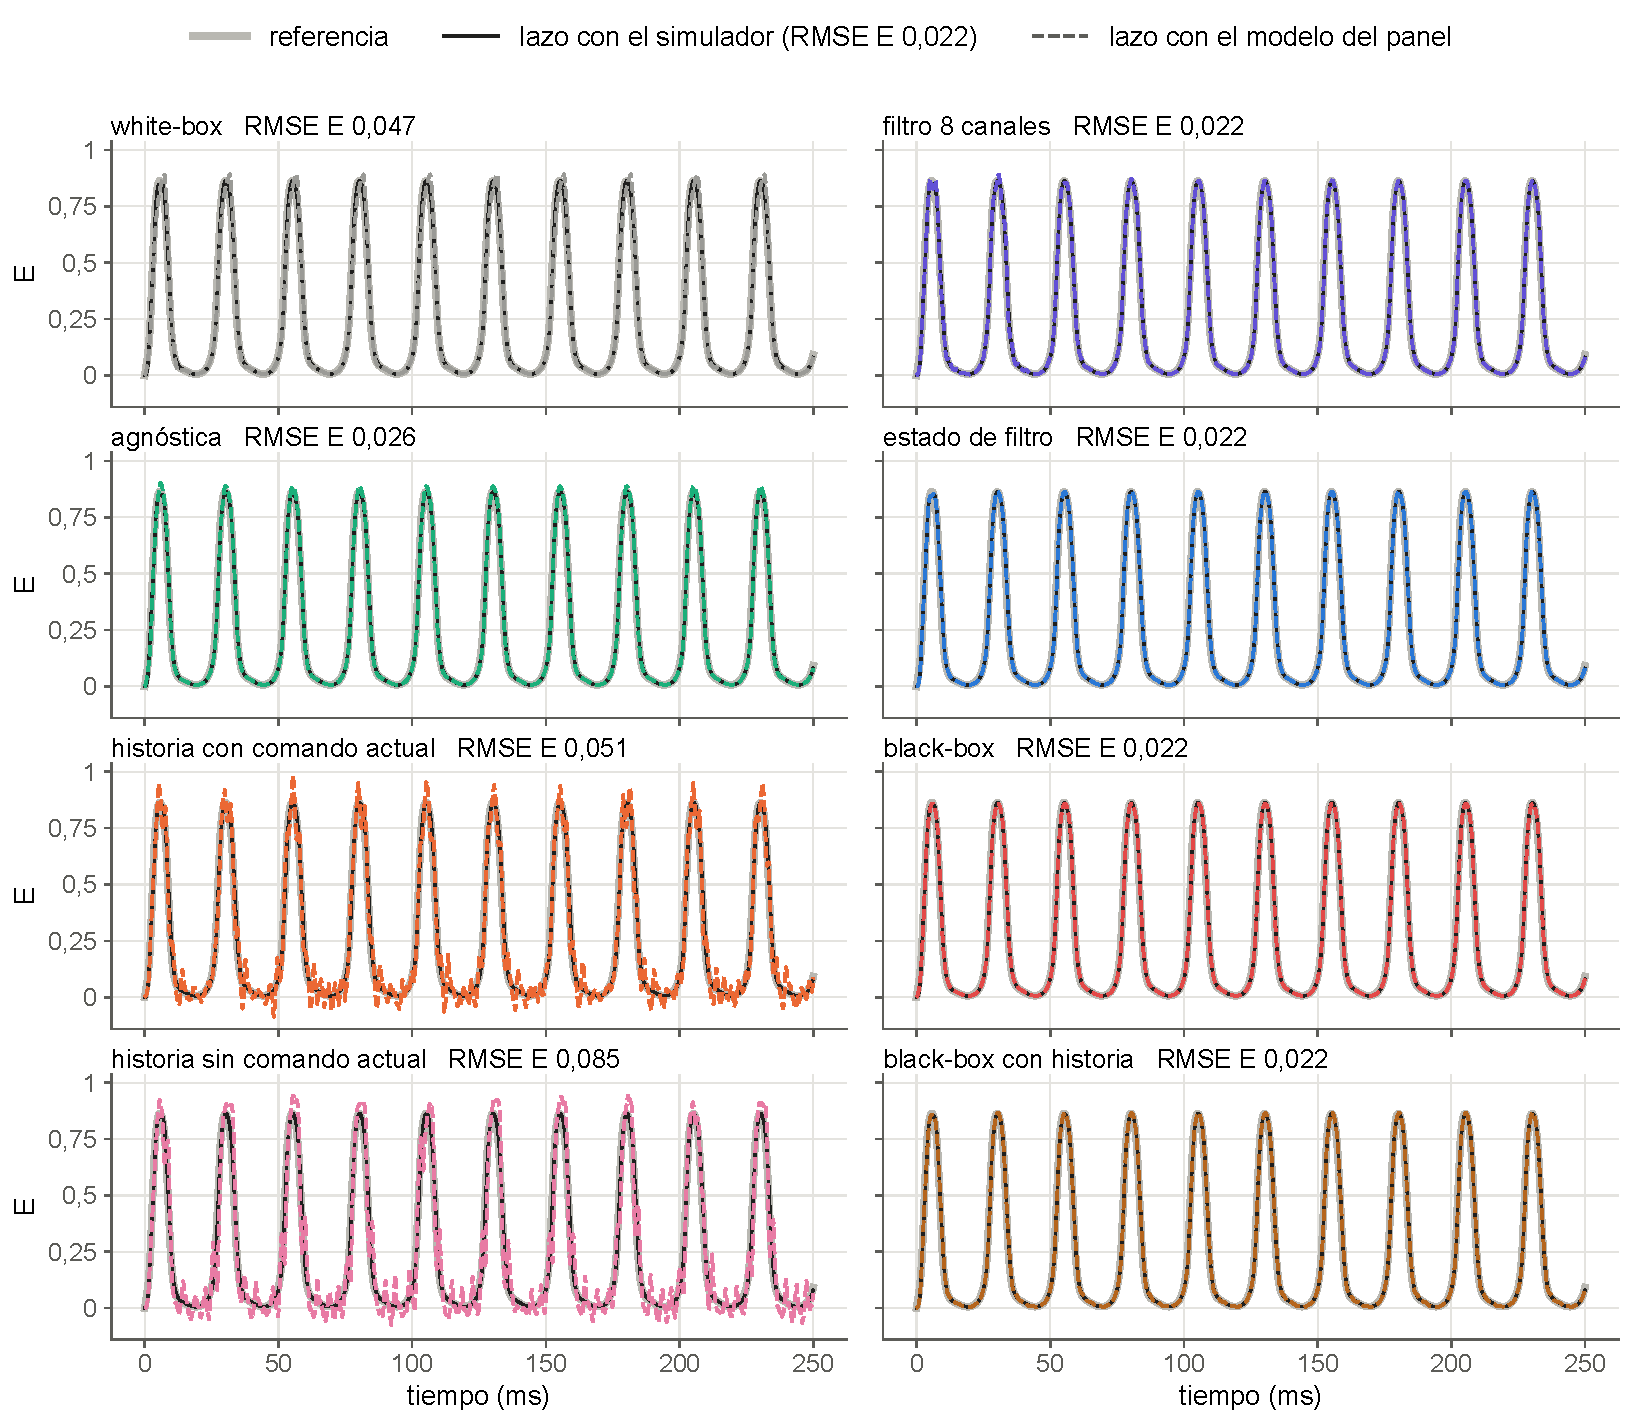
\includegraphics[width=\textwidth]{gamma_rango_E.pdf}
\caption{Actividad $E$ con la referencia gamma de 40~Hz en rango. Gris, referencia. Negro, lazo con el simulador. Discontinua, lazo con el modelo del panel, entrenado con amplitud grande (semilla 0, $\sigma = 0{,}01$). En cada panel, RMSE contra la referencia.}
\end{figure}
\begin{figure}[H]
\centering
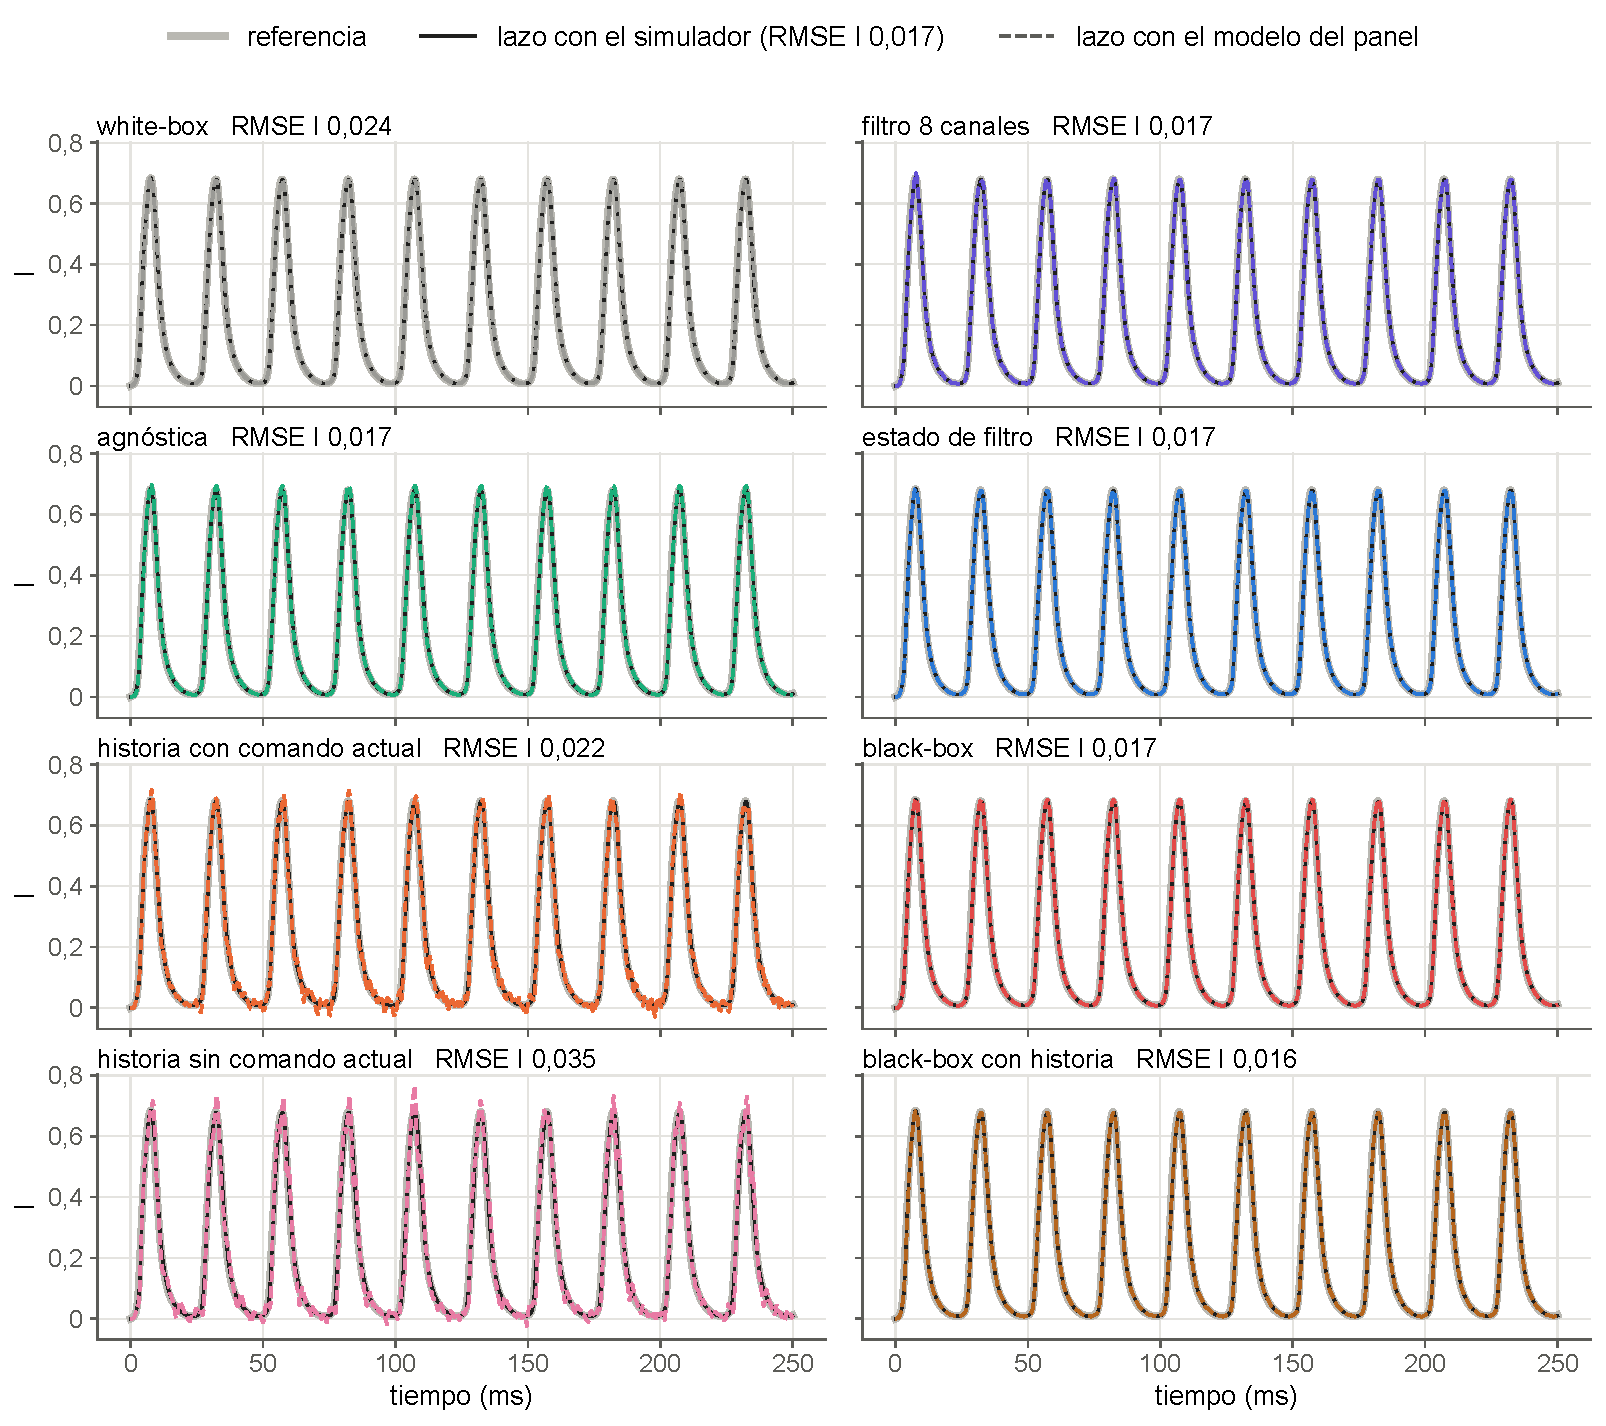
\includegraphics[width=\textwidth]{gamma_rango_I.pdf}
\caption{Actividad $I$ con la referencia gamma de 40~Hz en rango.}
\end{figure}
Con las referencias en rango, el estado de filtro, la black-box, la black-box con historia y el filtro de 8 canales siguen casi igual que el simulador. El white-box y la agnóstica quedan algo por encima. Las dos historias oscilan en los tramos de baja actividad, y la historia sin comando actual es la que más se aparta (RMSE de 0,073 contra 0,011 del simulador en la theta).


\section{Conclusiones}

\begin{itemize}[leftmargin=*,itemsep=0.4em]
\item Con comandos en el rango del controlador, la forma exacta de cada perturbación identifica todos sus parámetros, incluido el nivel del recorte, con errores de $\bh$ de 0,1 a 0,7~\%, y reproduce el lazo cerrado del simulador sin ajustes a mano.
\item En el actuador, los modelos sin el recorte en su estructura reproducen en lazo abierto con parámetros sin relación con los verdaderos (42 a 204~\% de error). La saturación activa se compensa deformando $\beta$. El warm start desde el white-box empeora esa deformación.
\item En la refractaria, la amplitud grande mejora la identificación de todos los modelos con corrección, y la agnóstica ya no necesita warm start.
\item El sesgo por ruido en el estado inicial de las ventanas casi desaparece, porque la respuesta crece mucho más que el ruido.
\item Ampliar el rango de entrenamiento no alcanza para que las correcciones con red reproduzcan el lazo del simulador fuera de las referencias en rango. La estructura del modelo pesa más que el rango de los datos.
\item La black-box con historia es la mejor sin forma exacta en lazo abierto del actuador, y en lazo cerrado queda como el white-box.
\end{itemize}

\section{Preguntas posibles}

\begin{preguntas}
\pr{¿Por qué el white-box empeora tanto en el actuador, si los datos son más ricos?}
Porque los datos nuevos muestran una saturación que el white-box no puede representar. Con comandos de hasta 12, el simulador recibe como máximo 3, y el white-box explica esa respuesta reducida bajando los pesos y corriendo los umbrales. Con los datos de $[0, 2]$ el recorte no actuaba y esa deformación no hacía falta.

\pr{¿Por qué el warm start empeora a las redes en el actuador?}
Porque arrancan del white-box, que ya tiene $\bh$ con 122~\% de error. La red aprende una corrección sobre esos parámetros y no los lleva de vuelta. Desde cero, parámetros y red se ajustan juntos y el error queda en 42 a 71~\%, que sigue siendo alto.

\pr{¿El nivel del recorte se identifica porque se inicializó cerca de 3?}
No. Se inicializa en 10, como antes. Con comandos de hasta 12, el recorte en 10 actúa en los escenarios de mayor amplitud, recibe gradiente, y baja hasta un valor entre 2,99 y 3,01 en todas las corridas.

\pr{¿Por qué el NRMSE del test anterior empeora en el white-box y la agnóstica?}
Ese test tiene comandos positivos de hasta 2, donde el recorte no actúa. Los parámetros deformados para el régimen saturado responden mal en ese régimen. Las correcciones con historia lo compensan en parte, y la forma exacta no tiene el problema.

\pr{¿Conviene entonces entrenar siempre con amplitud grande?}
Para la forma exacta y para la refractaria, sí. Para las correcciones con red en el actuador, la amplitud grande mejora la reproducción pero empeora los parámetros, porque deja ver una física que su estructura no tiene. El paper puede presentar las dos tandas como dos regímenes de identificación.

\pr{¿Por qué la black-box puede estar en el lazo cerrado ahora?}
Se agregó a la simulación del lazo el caso de un modelo sin backbone, donde el campo es solo la red. Se verificó que el campo calculado en la simulación coincide con el de PyTorch (diferencia relativa del orden de $10^{-7}$).
\end{preguntas}

\end{document}
